% Options for packages loaded elsewhere
\PassOptionsToPackage{unicode}{hyperref}
\PassOptionsToPackage{hyphens}{url}
\PassOptionsToPackage{dvipsnames,svgnames,x11names}{xcolor}
\documentclass[
  10pt,
  fontset=fandol]{ctexart}
\usepackage{xcolor}
\usepackage[margin=16mm]{geometry}
\usepackage{amsmath,amssymb}
\setcounter{secnumdepth}{-\maxdimen} % remove section numbering
\usepackage{iftex}
\ifPDFTeX
  \usepackage[T1]{fontenc}
  \usepackage[utf8]{inputenc}
  \usepackage{textcomp} % provide euro and other symbols
\else % if luatex or xetex
  \usepackage{unicode-math} % this also loads fontspec
  \defaultfontfeatures{Scale=MatchLowercase}
  \defaultfontfeatures[\rmfamily]{Ligatures=TeX,Scale=1}
\fi
\usepackage{lmodern}
\ifPDFTeX\else
  % xetex/luatex font selection
\fi
% Use upquote if available, for straight quotes in verbatim environments
\IfFileExists{upquote.sty}{\usepackage{upquote}}{}
\IfFileExists{microtype.sty}{% use microtype if available
  \usepackage[]{microtype}
  \UseMicrotypeSet[protrusion]{basicmath} % disable protrusion for tt fonts
}{}
\makeatletter
\@ifundefined{KOMAClassName}{% if non-KOMA class
  \IfFileExists{parskip.sty}{%
    \usepackage{parskip}
  }{% else
    \setlength{\parindent}{0pt}
    \setlength{\parskip}{6pt plus 2pt minus 1pt}}
}{% if KOMA class
  \KOMAoptions{parskip=half}}
\makeatother
\usepackage{longtable,booktabs,array}
\newcounter{none} % for unnumbered tables
\usepackage{calc} % for calculating minipage widths
% Correct order of tables after \paragraph or \subparagraph
\usepackage{etoolbox}
\makeatletter
\patchcmd\longtable{\par}{\if@noskipsec\mbox{}\fi\par}{}{}
\makeatother
% Allow footnotes in longtable head/foot
\IfFileExists{footnotehyper.sty}{\usepackage{footnotehyper}}{\usepackage{footnote}}
\makesavenoteenv{longtable}
\usepackage{graphicx}
\makeatletter
\newsavebox\pandoc@box
\newcommand*\pandocbounded[1]{% scales image to fit in text height/width
  \sbox\pandoc@box{#1}%
  \Gscale@div\@tempa{\textheight}{\dimexpr\ht\pandoc@box+\dp\pandoc@box\relax}%
  \Gscale@div\@tempb{\linewidth}{\wd\pandoc@box}%
  \ifdim\@tempb\p@<\@tempa\p@\let\@tempa\@tempb\fi% select the smaller of both
  \ifdim\@tempa\p@<\p@\scalebox{\@tempa}{\usebox\pandoc@box}%
  \else\usebox{\pandoc@box}%
  \fi%
}
% Set default figure placement to htbp
\def\fps@figure{htbp}
\makeatother
\setlength{\emergencystretch}{3em} % prevent overfull lines
\providecommand{\tightlist}{%
  \setlength{\itemsep}{0pt}\setlength{\parskip}{0pt}}
\usepackage{amsmath,amssymb,mathtools,needspace}
\xeCJKDeclareCharClass{CJK}{"2032,"0400->"04FF,"2160->"216B,"2460->"2473,"25A0,"25C7,"25CB,"25CF}
\IfFontExistsTF{Arial Unicode MS}{\xeCJKsetup{AutoFallBack=true}\setCJKfallbackfamilyfont{\CJKrmdefault}{Arial Unicode MS}}{}
\setcounter{secnumdepth}{0}
\setlength{\emergencystretch}{2em}
\allowdisplaybreaks
\usepackage{bookmark}
\IfFileExists{xurl.sty}{\usepackage{xurl}}{} % add URL line breaks if available
\urlstyle{same}
\hypersetup{
  pdftitle={数值微分},
  colorlinks=true,
  linkcolor={Maroon},
  filecolor={Maroon},
  citecolor={Blue},
  urlcolor={Blue},
  pdfcreator={LaTeX via pandoc}}

\title{数值微分}
\author{}
\date{}

\begin{document}
\maketitle

\subsection{4.5 数值微分}\label{ux6570ux503cux5faeux5206}

\subsubsection{4.5.1 中点方法}\label{ux4e2dux70b9ux65b9ux6cd5}

按照数学分析的定义，导数 \(f'(a)\) 是差商 \(\dfrac{f(a+h)-f(a)}h\) 当 \(h\to0\) 时的极限。如果精度要求不高，我们可以简单地取差商作为导数的近似值，这样便建立起一种数值微分方法，即

\[
f'(a)\approx\frac{f(a+h)-f(a)}h.
\]

类似地，亦可用向后差商作近似运算，即

\[
f'(a)\approx\frac{f(a)-f(a-h)}h
\]

或用中心差商作近似计算，即

\[
f'(a)\approx\frac{f(a+h)-f(a-h)}{2h}.
\]

后一种数值微分方法称中点方法，它其实是前两种方法的算术平均。

在图 4.3 上，上述三种导数的近似值分别表示弦线 \(AB\)、\(AC\) 和 \(BC\) 的斜率，比较这三种弦线与切线 \(AT\)（其斜率等于导数值 \(f'(a)\)）平行的程度，从图形上可以明显地看出，其中以 \(BC\) 的斜率更接近于切线 \(AT\) 的斜率。因此就精度而言，以中点方法更为可取。

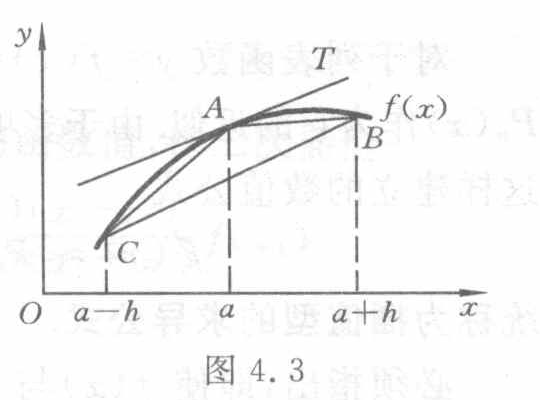
\includegraphics[width=0.85\linewidth,height=\textheight,keepaspectratio,alt={图 4.3（原书扫描裁切）}]{../assets/ch04b/figure-4-3.png}

图 4.3。原图标签：横轴 \(x\)、纵轴 \(y\)、原点 \(O\)；横轴位置 \(a-h\)、\(a\)、\(a+h\)，对应曲线上的点 \(C\)、\(A\)、\(B\)；曲线标记 \(f(x)\)，过 \(A\) 的切线标记 \(T\)。图中画出弦线 \(AB\)、\(AC\)、\(BC\) 与切线 \(AT\)。（此段为图中标签和图意的文字转录；原图未给出具体函数或数值。）

上述三种数值微分方法有个共同点，它们都是将导数的计算归结为计算 \(f\) 在若干节点上的函数值。这类数值微分方法称为机械求导方法。

要利用中点公式

\[
G(h)=\frac{f(a+h)-f(a-h)}{2h}
\]

计算导数 \(f'(a)\) 的近似值，首先必须选取合适的步长，为此需要进行误差分析。分别将 \(f(a\pm h)\) 在 \(x=a\) 处作 Taylor 展开，有

\[
f(a\pm h)=f(a)\pm hf'(a)+\frac{h^2}{2!}f''(a)
\pm\frac{h^3}{3!}f'''(a)+\frac{h^4}{4!}f^{(4)}(a)
\pm\frac{h^5}{5!}f^{(5)}(a)+\cdots,
\]

代入上式得

\[
G(h)=f'(a)+\frac{h^2}{3!}f'''(a)+\frac{h^4}{5!}f^{(5)}(a)+\cdots.
\]

\href{../../source-images/pdf-113.jpeg}{原页图像}

\subsubsection{4.5.1 中点方法（续）}\label{ux4e2dux70b9ux65b9ux6cd5ux7eed}

由此得知，从截断误差的角度看，步长越小，计算结果越准确。

再考察舍入误差，按中点公式计算。当 \(h\) 很小时，因 \(f(a+h)\) 与 \(f(a-h)\) 很接近，直接相减会造成有效数字的严重损失（参见 1.4 节）。因此，从舍入误差的角度来看，步长是不宜太小的。

例如，用中点公式求 \(f(x)=\sqrt{x}\) 在 \(x=2\) 处的一阶导数，有

\[
G(h)=\frac{\sqrt{2+h}-\sqrt{2-h}}{2h}.
\]

设取四位数字计算，结果如表 4.6（导数的准确值 \(f'(2)=0.353\,553\)）所示。

\textbf{表 4.6}

{\def\LTcaptype{none} % do not increment counter
\begin{longtable}[]{@{}rrrrrr@{}}
\toprule\noalign{}
\(h\) & \(G(h)\) & \(h\) & \(G(h)\) & \(h\) & \(G(h)\) \\
\midrule\noalign{}
\endhead
\bottomrule\noalign{}
\endlastfoot
\(1\) & \(0.366\,0\) & \(0.05\) & \(0.353\,0\) & \(0.001\) & \(0.350\,0\) \\
\(0.5\) & \(0.356\,4\) & \(0.01\) & \(0.350\,0\) & \(0.000\,5\) & \(0.300\,0\) \\
\(0.1\) & \(0.353\,5\) & \(0.005\) & \(0.350\,0\) & \(0.000\,1\) & \(0.300\,0\) \\
\end{longtable}
}

在表 4.6 中，\(h=0.1\) 的逼近效果最好，如果进一步缩小步长，则逼近的效果会越来越差。

\subsubsection{4.5.2 插值型的求导公式}\label{ux63d2ux503cux578bux7684ux6c42ux5bfcux516cux5f0f}

对于列表函数 \(y=f(x)\)（见表 4.7），运用插值原理，可以建立插值多项式 \(y=P_n(x)\) 作为它的近似。由于多项式的求导比较容易，取 \(P_n'(x)\) 的值作为 \(f'(x)\) 的近似值，这样建立的数值公式

\[
f'(x)\approx P_n'(x)
\tag{4.5.1}
\]

统称为插值型的求导公式。

\textbf{表 4.7}

{\def\LTcaptype{none} % do not increment counter
\begin{longtable}[]{@{}cccccc@{}}
\toprule\noalign{}
\(x\) & \(x_0\) & \(x_1\) & \(x_2\) & \(\cdots\) & \(x_n\) \\
\midrule\noalign{}
\endhead
\bottomrule\noalign{}
\endlastfoot
\(y\) & \(y_0\) & \(y_1\) & \(y_2\) & \(\cdots\) & \(y_n\) \\
\end{longtable}
}

必须指出，即使 \(f(x)\) 与 \(P_n(x)\) 的值相差不多，导数的近似值 \(P_n'(x)\) 与导数的真值 \(f'(x)\) 仍然可能差别很大，因而在使用求导公式（4.5.1）时应特别注意误差的分析。

依据插值余项定理，求导公式（4.5.1）的余项为

\[
f'(x)-P_n'(x)=\frac{f^{(n+1)}(\xi)}{(n+1)!}\omega_{n+1}'(x)
+\frac{\omega_{n+1}(x)}{(n+1)!}\frac{\mathrm{d}}{\mathrm{d}x}f^{(n+1)}(\xi),
\]

其中

\[
\omega_{n+1}(x)=\prod_{k=0}^{n}(x-x_i).
\]

在此余项公式中，由于 \(\xi\) 是 \(x\) 的未知函数，无法对其第二项 \(\dfrac{\omega_{n+1}(x)}{(n+1)!}\dfrac{\mathrm{d}}{\mathrm{d}x}f^{(n+1)}(\xi)\) 作出进一步的说明，因此，对于随意给出的点 \(x\)，误差 \(f'(x)-P_n'(x)\) 是无法预估的。但是，如果限定求某个节点 \(x_k\) 上的导数值，那么上面的第二项因 \(\omega_{n+1}(x_k)=0\) 而变为

（本句续下页。）

\begin{quote}
校注（agent 补充，CH04B-E004）：原页``其中''后的节点多项式印为 \(\prod_{k=0}^{n}(x-x_i)\)，乘积指标 \(k\) 与因子下标 \(i\) 不一致，已按原扫描保留。结合本页表 4.7 和下文 \(\omega_{n+1}(x_k)=0\)，应将因子写作 \((x-x_k)\)，或统一将乘积指标改为 \(i\)；这是原书疑似下标排印错误，非 OCR 错误。\href{../assets/ch04b/review-p113-product.png}{局部原扫描}。
\end{quote}

\href{../../source-images/pdf-114.jpeg}{原页图像}

\subsubsection{4.5.2 插值型的求导公式（续）}\label{ux63d2ux503cux578bux7684ux6c42ux5bfcux516cux5f0fux7eed}

零，这时有余项公式

\[
f'(x_k)-P_n'(x_k)=\frac{f^{(n+1)}(\xi)}{(n+1)!}\omega_{n+1}'(x_k).
\tag{4.5.2}
\]

下面仅仅考察节点处的导数值。为简化讨论，假定所给的节点是等距的。

\paragraph{1. 两点公式}\label{ux4e24ux70b9ux516cux5f0f}

设已给出两个节点 \(x_0,x_1\) 上面的函数值 \(f(x_0),f(x_1)\)，作线性插值公式

\[
P_1(x)=\frac{x-x_1}{x_0-x_1}f(x_0)+\frac{x-x_0}{x_1-x_0}f(x_1).
\]

对上式两端求导，记 \(x_1-x_0=h\)，有

\[
P_1'(x)=\frac1h[-f(x_0)+f(x_1)],
\]

于是有下列求导公式：

\[
P_1'(x_0)=\frac1h[f(x_1)-f(x_0)],\quad
P_1'(x_1)=\frac1h[f(x_1)-f(x_0)].
\]

而利用余项公式（4.5.2）知，带余项的两点公式是

\[
f'(x_0)=\frac1h[f(x_1)-f(x_0)]-\frac h2f''(\xi),
\]

\[
f'(x_1)=\frac1h[f(x_1)-f(x_0)]+\frac h2f''(\xi).
\]

\paragraph{2. 三点公式}\label{ux4e09ux70b9ux516cux5f0f}

设已给出三个节点 \(x_0,x_1=x_0+h,x_2=x_0+2h\) 上的函数值，作二次插值

\[
\begin{aligned}
P_2(x)={}&\frac{(x-x_1)(x-x_2)}{(x_0-x_1)(x_0-x_2)}f(x_0)
+\frac{(x-x_0)(x-x_2)}{(x_1-x_0)(x_1-x_2)}f(x_1)\\
&+\frac{(x-x_0)(x-x_1)}{(x_2-x_0)(x_2-x_1)}f(x_2),
\end{aligned}
\]

令 \(x=x_0+th\)，上式可表示为

\[
P_2(x_0+th)=\frac12(t-1)(t-2)f(x_0)-t(t-2)f(x_1)
+\frac12t(t-1)f(x_2),
\]

两端对 \(t\) 求导，有

\[
P_2'(x_0+th)=\frac1{2h}[(2t-3)f(x_0)-(4t-4)f(x_1)+(2t-1)f(x_2)].
\tag{4.5.3}
\]

这里撇号表示对变量 \(x\) 求导数。上式分别取 \(t=0,1,2\)，得到以下三种三点公式：

\[
P_2'(x_0)=\frac1{2h}[-3f(x_0)+4f(x_1)-f(x_2)],
\]

\[
P_2'(x_1)=\frac1{2h}[-f(x_0)+f(x_2)],
\]

（第三个公式续下页。）

\href{../../source-images/pdf-115.jpeg}{原页图像}

\subsubsection{4.5.2 插值型的求导公式（续）}\label{ux63d2ux503cux578bux7684ux6c42ux5bfcux516cux5f0fux7eed-1}

\paragraph{2. 三点公式（续）}\label{ux4e09ux70b9ux516cux5f0fux7eed}

\[
P_2'(x_2)=\frac1{2h}[f(x_0)-4f(x_1)+3f(x_2)],
\]

而带余项的三点求导公式为

\[
f'(x_0)=\frac1{2h}[-3f(x_0)+4f(x_1)-f(x_2)]+\frac{h^2}3f'''(\xi),
\]

\[
f'(x_1)=\frac1{2h}[-f(x_0)+f(x_2)]-\frac{h^2}6f'''(\xi),
\tag{4.5.4}
\]

\[
f'(x_2)=\frac1{2h}[f(x_0)-4f(x_1)+3f(x_2)]+\frac{h^2}3f'''(\xi),
\]

其中式（4.5.4）是我们所熟悉的中点公式。在三点公式中，它由于少用了一个函数值 \(f(x_1)\) 而引人注目。

用插值多项式 \(P_n(x)\) 作为 \(f(x)\) 的近似函数，还可以建立高阶数值微分公式

\[
f^{(k)}(x)\approx P_n^{(k)}(x),\quad k=1,2,\cdots.
\]

例如，将式（4.5.3）再对 \(t\) 求导一次，有

\[
P_2''(x_0+th)=\frac1{h^2}[f(x_0)-2f(x_1)+f(x_2)],
\]

于是有

\[
P_2''(x_1)=\frac1{h^2}[f(x_1-h)-2f(x_1)+f(x_1+h)],
\]

而带余项的二阶三点公式为

\[
f''(x_1)=\frac1{h^2}[f(x_1-h)-2f(x_1)+f(x_1+h)]-\frac{h^2}{12}f^{(4)}(\xi).
\tag{4.5.5}
\]

\subsubsection{4.5.3 实用的五点公式}\label{ux5b9eux7528ux7684ux4e94ux70b9ux516cux5f0f}

设已给出五个节点 \(x_i=x_0+ih,\allowbreak \quad i=0,\allowbreak 1,\allowbreak 2,\allowbreak 3,\allowbreak 4\) 上的函数值，重复同样的手续，不难导出下列五点公式：

\[
m_0=\frac1{12h}[-25f(x_0)+48f(x_1)-36f(x_2)+16f(x_3)-3f(x_4)],
\]

\[
m_1=\frac1{12h}[-3f(x_0)-10f(x_1)+18f(x_2)-6f(x_3)+f(x_4)],
\]

\[
m_2=\frac1{12h}[f(x_0)-8f(x_1)+8f(x_3)-f(x_4)],
\]

\[
m_3=\frac1{12h}[-f(x_0)+6f(x_1)-18f(x_2)+10f(x_3)+3f(x_4)],
\]

\[
m_4=\frac1{12h}[3f(x_0)-16f(x_1)+36f(x_2)-48f(x_3)+25f(x_4)].
\]

其中 \(m_i\) 代表一阶导数 \(f'(x_i)\) 的近似值，读者不难导出这些求导公式的余项。

再记 \(M_i\) 表示二阶导数 \(f''(x_i)\) 的近似值，二阶五点公式如下：

（公式续下页。）

\href{../../source-images/pdf-116.jpeg}{原页图像}

\subsubsection{4.5.3 实用的五点公式（续）}\label{ux5b9eux7528ux7684ux4e94ux70b9ux516cux5f0fux7eed}

\[
M_0=\frac1{12h^2}[35f(x_0)-104f(x_1)+114f(x_2)-56f(x_3)+11f(x_4)],
\]

\[
M_1=\frac1{12h^2}[11f(x_0)-20f(x_1)+6f(x_2)+4f(x_3)-f(x_4)],
\]

\[
M_2=\frac1{12h^2}[-f(x_0)+16f(x_1)-30f(x_2)+16f(x_3)-f(x_4)],
\]

\[
M_3=\frac1{12h^2}[-f(x_0)+4f(x_1)+6f(x_2)-20f(x_3)+11f(x_4)],
\]

\[
M_4=\frac1{12h^2}[11f(x_0)-56f(x_1)+114f(x_2)-104f(x_3)+35f(x_4)].
\]

对于给定的一张数据表，用五点公式求节点上的导数值往往可以获得满意的结果。五个相邻节点的选择原则，一般是在所考察的节点的两侧各取两个邻近的节点，如果一侧的节点数不足两个（即一侧只有一个节点或没有节点），则用另一侧的节点补足。

\textbf{例 4.4}　利用 \(f(x)=\sqrt{x}\) 的一张数据表，按五点公式求节点上的导数值 \(m_i\) 与 \(M_i\)，并与导数的准确值比较，如表 4.8 所示。

\textbf{表 4.8}

{\def\LTcaptype{none} % do not increment counter
\begin{longtable}[]{@{}
  >{\raggedleft\arraybackslash}p{(\linewidth - 10\tabcolsep) * \real{0.1667}}
  >{\raggedleft\arraybackslash}p{(\linewidth - 10\tabcolsep) * \real{0.1667}}
  >{\raggedleft\arraybackslash}p{(\linewidth - 10\tabcolsep) * \real{0.1667}}
  >{\raggedleft\arraybackslash}p{(\linewidth - 10\tabcolsep) * \real{0.1667}}
  >{\raggedleft\arraybackslash}p{(\linewidth - 10\tabcolsep) * \real{0.1667}}
  >{\raggedleft\arraybackslash}p{(\linewidth - 10\tabcolsep) * \real{0.1667}}@{}}
\toprule\noalign{}
\begin{minipage}[b]{\linewidth}\raggedleft
\(x_i\)
\end{minipage} & \begin{minipage}[b]{\linewidth}\raggedleft
\(f(x_i)\)
\end{minipage} & \begin{minipage}[b]{\linewidth}\raggedleft
\(m_i\)
\end{minipage} & \begin{minipage}[b]{\linewidth}\raggedleft
\(f'(x_i)\)
\end{minipage} & \begin{minipage}[b]{\linewidth}\raggedleft
\(M_i/\times10^3\)
\end{minipage} & \begin{minipage}[b]{\linewidth}\raggedleft
\(f''(x_i)/\times10^3\)
\end{minipage} \\
\midrule\noalign{}
\endhead
\bottomrule\noalign{}
\endlastfoot
\(100\) & \(10.000\,000\) & \(0.050\,000\) & \(0.050\,000\) & \(-0.247\,58\) & \(-0.250\,00\) \\
\(101\) & \(10.049\,875\) & \(0.049\,751\) & \(0.049\,752\) & \(-0.245\,91\) & \(-0.246\,30\) \\
\(102\) & \(10.099\,504\) & \(0.049\,507\) & \(0.049\,507\) & \(-0.241\,91\) & \(-0.242\,68\) \\
\(103\) & \(10.148\,891\) & \(0.049\,267\) & \(0.049\,266\) & \(-0.239\,58\) & \(-0.239\,16\) \\
\(104\) & \(10.198\,039\) & \(0.049\,029\) & \(0.049\,029\) & \(-0.236\,91\) & \(-0.235\,72\) \\
\(105\) & \(10.246\,950\) & \(0.048\,795\) & \(0.048\,795\) & \(-0.236\,66\) & \(-0.232\,36\) \\
\end{longtable}
}

\subsubsection{4.5.4 样条求导}\label{ux6837ux6761ux6c42ux5bfc}

我们知道，样条函数 \(S(x)\) 作为 \(f(x)\) 的近似函数，不但彼此的函数值很接近，导数值也很接近。例如，对于三次样条 \(S_3(x)\)，有

\[
|f^{(a)}(x)-S_3^{(a)}(x)|=O(h^{4-a})\qquad(a=0,1,2,3),
\]

因此，用样条函数建立数值微分公式是很自然的，即

\[
f^{(a)}(x)\approx S_3^{(a)}(x)\qquad(a=0,1,2,3).
\tag{4.5.6}
\]

与前述插值型微分公式（4.5.1）不同，样条微分公式（4.5.6）可以用来计算插值范围内任何一点 \(x\)（不仅是节点 \(x_i\)）上的导数值。对于等距分划

\[
\pi:a=x_0<x_1<x_2<\cdots<x_n=b,\quad x_{k+1}-x_k=h,
\]

三次样条 \(S_3(x)\) 在节点上的导数值 \(S_3'(x_k)=m_k\) 满足下列连续性方程组

（方程组续下页。）

\begin{quote}
校注（agent 补充，原表记法说明）：表 4.8 后两列表头按原扫描保留为 \(M_i/\times10^3\) 与 \(f''(x_i)/\times10^3\)，未改写原表头。表内数值对应导数乘 \(10^3\) 后的数值，例如 \(f''(100)=-1/(4\cdot100^{3/2})=-0.00025\)，表中列为 \(-0.25000\)；此说明仅解释该页缩放记法。\href{../assets/ch04b/review-table-4-8.png}{表 4.8 原扫描局部}。
\end{quote}

\href{../../source-images/pdf-117.jpeg}{原页图像}

\subsubsection{4.5.4 样条求导（续）}\label{ux6837ux6761ux6c42ux5bfcux7eed}

\[
m_{k-1}+4m_k+m_{k+1}=3(y_{k+1}-y_{k-1})/h,\quad k=1,2,\cdots,n-1.
\tag{4.5.7}
\]

设已给出端点处的一阶导数值 \(m_0=y_0',m_n=y_n'\)，则求解方程组（4.5.7）得出的 \(m_k\) 即可作为导数 \(f'(x_k)\) 的近似值。

\begin{center}\rule{0.5\linewidth}{0.5pt}\end{center}

\subsection{相关原页校注（agent 补充）}\label{ux76f8ux5173ux539fux9875ux6821ux6ce8agent-ux8865ux5145}

以下校注来自本节覆盖的原页，可能也涉及同页相邻小节；原文照录与校正说明分开保留。

\subsubsection{原书 PDF 页 117 的校注}\label{ux539fux4e66-pdf-ux9875-117-ux7684ux6821ux6ce8}

\href{../pages/pdf-117.md}{完整原页转录} · \href{../../source-images/pdf-117.jpeg}{原页图像}

校注记录：CH04B-E005。

\begin{quote}
校注（agent 补充，CH04B-E005）：第 1 题（4）首项的分母在原扫描中明确印为``1''，故保留 \(h[f(0)+f(h)]/1\)。该处疑为原书排印错误：仅作排印一致性检查，当 \(f\equiv1\) 时，积分为 \(h\)，而所印右端为 \(2h\)，并且导数项为零；疑应将分母印为``2''。此处不求解题中参数或代数精度。\href{../assets/ch04b/review-p117-exercises.png}{习题原扫描局部}。
\end{quote}

\subsection{本节覆盖原页的校注记录}\label{ux672cux8282ux8986ux76d6ux539fux9875ux7684ux6821ux6ce8ux8bb0ux5f55}

下列记录按原页关联，含同页相邻小节的校注；计算时同时读取上文校注和完整原页。

\begin{itemize}
\tightlist
\item
  \texttt{CH04B-E004}：原书 PDF 页 113
\item
  \texttt{CH04B-E005}：原书 PDF 页 117
\end{itemize}

\end{document}
